\subsection{Logging}
\label{section:process-logging}
We log using JSON, which allows us to select specific fields to display in Kibana, making the logs easy to read, filter, and sort by. \autoref{fig:logs-example} shows how we display logs in an easy-to-read format.
\begin{figure}[H]
  \makebox[\textwidth][c]{
    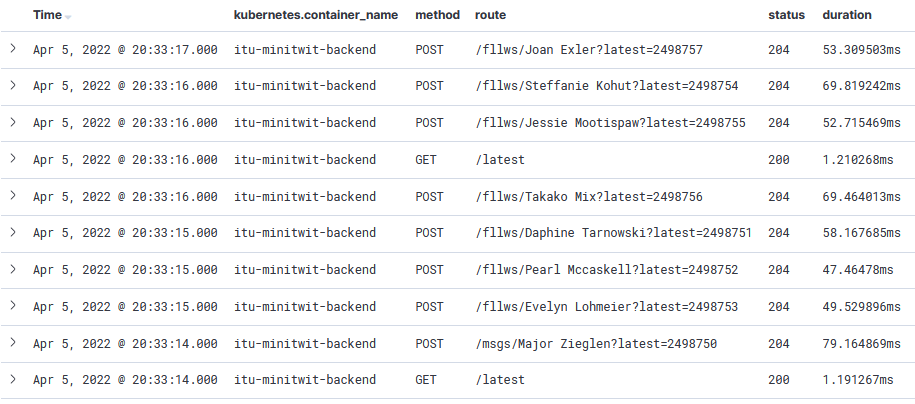
\includegraphics[width=0.9\paperwidth]{kibana-logs-structure.png}
  }
  \caption{Example of how we view logs in Kibana.}
  \label{fig:logs-example}
\end{figure}
It's not shown on the figure, but we also have a column for error messages, which we've experienced makes it easy to diagnose problems in the system. To diagnose performance issues, the ``duration'' column has also been helpful. By the end of the project, the mentioned log output has been enough to diagnose bugs and get an overview of what's happening in the system.
